% vim: spell spl=pt fo+=tcwa tw=98 nonu fdc=0
% vim: ts=4 sw=4 sts=4 expandtab
\documentclass{beamer}
\usepackage[brazil]{babel}
\usepackage[utf8]{inputenc}
\usepackage[T1]{fontenc}
\usepackage{graphicx,epstopdf,wrapfig,caption,url}

\title[MIHS]{Transições Interrede Independentes do Meio Físico de Acesso}
\author{Higor Eurípedes P. F. A.}
\institute[IFTO]{Instituto Federal de Educação, Ciência e Tecnologia do Tocantins}
\date[Março 2012]{16 de março de 2012}

%\AtBeginSection[]
%{
%  \begin{frame}
%    \frametitle{\secname}
%    \tableofcontents[currentsection,currentsubsection]
%  \end{frame}
%}
%\AtBeginSubsection[]
%{
%  \begin{frame}
%    \frametitle{\secname}
%    \tableofcontents[currentsection,currentsubsection]
%  \end{frame}
%}

\usetheme{default}
\usecolortheme{seahorse}

\begin{document}
    \frame{\titlepage}

    \section{\inserttitle}

    \subsection{O projeto}
    \frame{
        \frametitle{\insertsectionhead}
        \framesubtitle{\insertsubsectionhead}

        \begin{block}{Problema}
        \end{block}

        \pause

        \begin{block}{Justificativa}
        \end{block}
        
        \pause

        \begin{block}{Objetivos}
        \end{block}
        
        \pause
        \begin{block}{Método}
        \end{block}
    }
   

    \subsection{Trabalhos relacionados}
    \frame{
        \frametitle{\insertsectionhead}
        \framesubtitle{\insertsubsectionhead}
       
        \begin{block}{Trabalhos relacionados}
            \begin{itemize}

                \item Tawil, R. et al (2008). Distributed handoff decision scheme using MIH 
                    function for the 4th generation wireless networks.
                \item Tainiuchi, K. et al (2009). IEEE 802.21: Media independent Features, 
                    applicability, and realization.
                \item Machań, P. et al (2008). Performance of mobility support mechanisms in a 
                    heterogeneous UMTS and IEEE 802.11 network offered under the IEEE 802.21 
                    standard.

            \end{itemize}
        \end{block}
    }
    

    \frame{
        \frametitle{\insertsectionhead}
        \framesubtitle{\insertsubsectionhead}

        \begin{figure}[ht]
            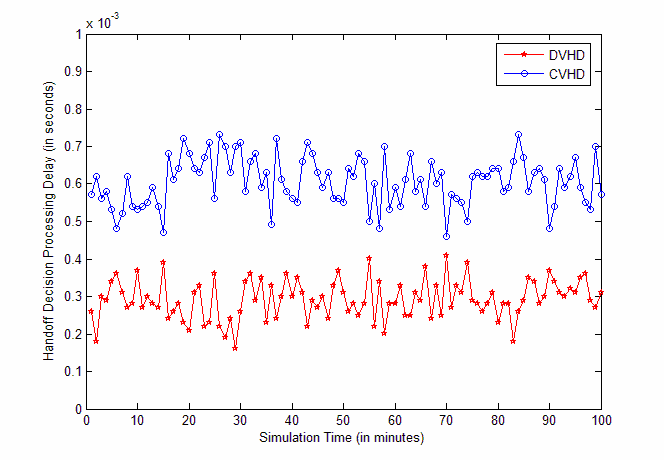
\includegraphics[width=.9\textwidth]{apresentacao-pre-projeto/dvhds-procdelay.png}
            \caption{Tempo de processamento de decisão. (Tawil)}
        \end{figure}
    }
    
    \frame{
        \frametitle{\insertsectionhead}
        \framesubtitle{\insertsubsectionhead}

        \begin{figure}[ht]
            \includegraphics[width=.9\textwidth]{apresentacao-pre-projeto/machan.eps}
            \caption{Tempo de \textit{handover} em relação à carga de rede. (Machań)}
        \end{figure}
    }

    
    \subsection{Proposta preliminar}
    \frame{
        \frametitle{\insertsectionhead}
        \framesubtitle{\insertsubsectionhead}

        \begin{block}{\subsecname}

            \begin{figure}
                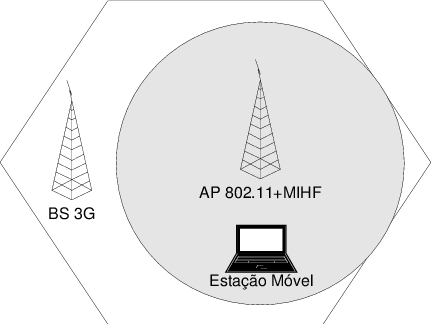
\includegraphics[width=.6\textwidth]{apresentacao-pre-projeto/ambiente.eps}
                \caption{Cenário proposto.}
            \end{figure}

        \end{block}
    }

    \frame{
        \frametitle{\insertsectionhead}
        \framesubtitle{\insertsubsectionhead}

        \begin{block}{Primitivas}
            \begin{table}[h!]
                \resizebox{\textwidth}{!}{
                    \begin{tabular}[b]{ l | l | l }
                        Primitiva & Serviço & Descrição \\
                        \hline
                        MIH\_Link\_Up          & MIES & O link está disponível. \\
                        MIH\_Link\_Down        & MIES & O link está indisponível. \\
                        MIH\_Link\_Going\_Down & MIES & O link poderá cair em breve. \\
                        MIH\_Link\_Switch      & MICS & Realiza o \textit{handover}. \\
                         MIH\_Report           & MICS & Obtém informações sobre uma estação. \\
                              MIH\_Discovery   & MIIS & Procura MIHFs servidoras na rede.  \\
                        \hline
                    \end{tabular}
                }
            \end{table}
            
        \end{block}
    } 

    \subsection{Conclusão}
    \frame{
        \frametitle{\insertsectionhead}
        \framesubtitle{\insertsubsectionhead}
       
        \begin{block}{Resultados esperados}
        \end{block}

        \pause
        
        \begin{block}{Conclusão}
        \end{block}
    }
    
\end{document}

